\section{BioClinical ModernBERT Appendix}
\label{app:bcb_supporting_tables}

Table~\ref{tab:bcb_appendix_stage1} records the key preprocessing and Stage~1 optimisation settings that supported the main BioClinical ModernBERT pipeline. Table~\ref{tab:bcb_appendix_stage2} records the detailed Stage~2 semi-supervised settings used for pseudo-label selection, student training, and the optional reasoning fallback. Table~\ref{tab:bcb_result_diagnostics} summarises the most important supporting diagnostics behind the final comparison, and Table~\ref{tab:bcb_final_confusion} gives the final official test confusion matrix for the selected calibrated committee.

\begin{table}[htbp]
\centering
\footnotesize
\setlength{\tabcolsep}{4pt}
\renewcommand{\arraystretch}{1.1}
\begin{tabularx}{\columnwidth}{|l|X|}
\hline
\textbf{Quantity} & \textbf{Value} \\
\hline
Labels & no=0, maybe=1, yes=2 \\
\hline
Input format & QUESTION + CONTEXTS \\
\hline
Truncation & only\_second \\
\hline
Max length & 512 \\
\hline
Mean length & 302.08 \\
\hline
Median length & 300 \\
\hline
95th percentile & 443.05 \\
\hline
99th percentile & 538.02 \\
\hline
Examples $>512$ & 90 / 5000 (1.80\%) \\
\hline
Backbone & BioClinical ModernBERT \\
\hline
Best imbalance method & weighted sampler only \\
\hline
Class-weighted loss & no \\
\hline
Supervised learning rate & $8\times10^{-6}$ \\
\hline
Gradient accumulation & 2 \\
\hline
Padding & dynamic \\
\hline
Model selection & validation macro F1 \\
\hline
Weak-stage labels & binary yes/no \\
\hline
Weak-stage pilot split & 10\% subset \\
\hline
Weak-stage best learning rate & $1\times10^{-5}$ \\
\hline
Weak-stage exported output & encoder only \\
\hline
\end{tabularx}
\caption{Supporting preprocessing and Stage~1 settings for BioClinical ModernBERT.}
\label{tab:bcb_appendix_stage1}
\end{table}

\begin{table}[htbp]
\centering
\footnotesize
\setlength{\tabcolsep}{4pt}
\renewcommand{\arraystretch}{1.1}
\begin{tabularx}{\columnwidth}{|l|X|}
\hline
\textbf{Quantity} & \textbf{Value} \\
\hline
Teacher agreement required & yes \\
\hline
Two-teacher purpose & diversity for agreement-based pseudo-label filtering \\
\hline
Confidence threshold (no, yes) & 0.78 \\
\hline
Margin threshold (no, yes) & 0.12 \\
\hline
Confidence threshold (maybe) & 0.62 \\
\hline
Margin threshold (maybe) & 0.05 \\
\hline
Pseudo-label multiplier & $2.5\times$ training fold \\
\hline
Typical pseudo-label target (i.e. number of pseudo-labels per student fold) & 1028 \\
\hline
Typical pseudo-label target (no) & 338 \\
\hline
Typical pseudo-label target (maybe) & 138 \\
\hline
Typical pseudo-label target (yes) & 552 \\
\hline
Maybe boost & 25\% \\
\hline
Pseudo-label type & soft labels \\
\hline
Pseudo-label loss weight & 0.35 \\
\hline
Student learning rate & $6\times10^{-6}$ \\
\hline
Student epochs & up to 6 \\
\hline
Student weighted sampling (off as it comes with own \\ method of handling maybe imbalance)   & off \\
\hline
Calibration purpose & soften overconfident probabilities before thresholding and ensembling \\
\hline
Final committee size & 10 \\
\hline
Committee voting rule & soft voting to preserve calibrated probabilities and reduce variance \\
\hline
Selective fallback trigger: confidence & $<0.55$ \\
\hline
Selective fallback trigger: top-two margin & $<0.22$ \\
\hline
Selective fallback budget & 20\% of test set \\
\hline
Reasoning model & BioMed-R1-8B \\
\hline
Fallback purpose & escalate only very low-confidence committee cases to reasoning model \\
\hline
Decoding & deterministic \\
\hline
Max new tokens & 128 \\
\hline
Prompt max length & 2048 \\
\hline
Few-shot examples in prompt & 3 (one per class) \\
\hline
Fallback if parse fails & original committee prediction \\
\hline
\end{tabularx}
\caption{Supporting Stage~2 semi-supervised and post-selection settings for BioClinical ModernBERT.}
\label{tab:bcb_appendix_stage2}
\end{table}

\begin{table}[htbp]
\centering
\footnotesize
\setlength{\tabcolsep}{4pt}
\renewcommand{\arraystretch}{1.1}
\begin{tabularx}{\columnwidth}{|X|c|c|}
\hline
\textbf{Quantity} & \textbf{Pipeline S} & \textbf{Pipeline E} \\
\hline
Mean outer accuracy & $0.712\pm0.038$ & $0.740\pm0.044$ \\
\hline
Mean outer macro F1 & $\mathbf{0.581\pm0.050}$ & $0.578\pm0.076$ \\
\hline
Mean outer F1\textsubscript{maybe} & $\mathbf{0.208\pm0.129}$ & $0.185\pm0.160$ \\
\hline
Best fold macro F1 & 0.680 (fold 7) & 0.702 (fold 2) \\
\hline
Simple-pipeline temperature range & 0.762--1.981 & -- \\
\hline
Final committee temperature range & 0.948--2.152 & -- \\
\hline
Selected pseudo-label count & -- & 578--1028 \\
\hline
Key pseudo-label failure & -- & fold 3: 0 \textit{no}, 26 \textit{maybe} candidates \\
\hline
\end{tabularx}
\caption{Compact supporting diagnostics for BioClinical ModernBERT.}
\label{tab:bcb_result_diagnostics}
\end{table}

\begin{table}[htbp]
\centering
\footnotesize
\setlength{\tabcolsep}{6pt}
\renewcommand{\arraystretch}{1.1}
\begin{tabular}{|l|c|c|c|}
\hline
\textbf{True class} & \textbf{Pred no} & \textbf{Pred maybe} & \textbf{Pred yes} \\
\hline
No & 120 & 21 & 28 \\
\hline
Maybe & 16 & 8 & 31 \\
\hline
Yes & 25 & 28 & 223 \\
\hline
\end{tabular}
\caption{Final test confusion matrix for the Pipeline S calibrated committee. Rows are true labels and columns are predicted labels.}
\label{tab:bcb_final_confusion}
\end{table}


\subsection{BioClinical ModernBERT training schematics}
\label{app:bcb_schematics}

Figures~\ref{fig:app_stage1_bcb} and~\ref{fig:app_stage2_bcb} summarise the final BioClinical ModernBERT training design. The Stage~1 schematic shows the route-selection process: masked adaptation on unlabelled data was tested but rejected, and the stronger base classifier route was then warm-started on the PQA-A weak-label set. The Stage~2 schematic shows the standardised 500/500 expert split, the outer 10-fold cross-validation protocol, the comparison between the simple supervised and advanced semi-supervised pipelines, and the final calibrated committee evaluation on the untouched test set.

\begin{figure}[H]
    \centering
    \begin{subfigure}[t]{0.47\linewidth}
        \centering
        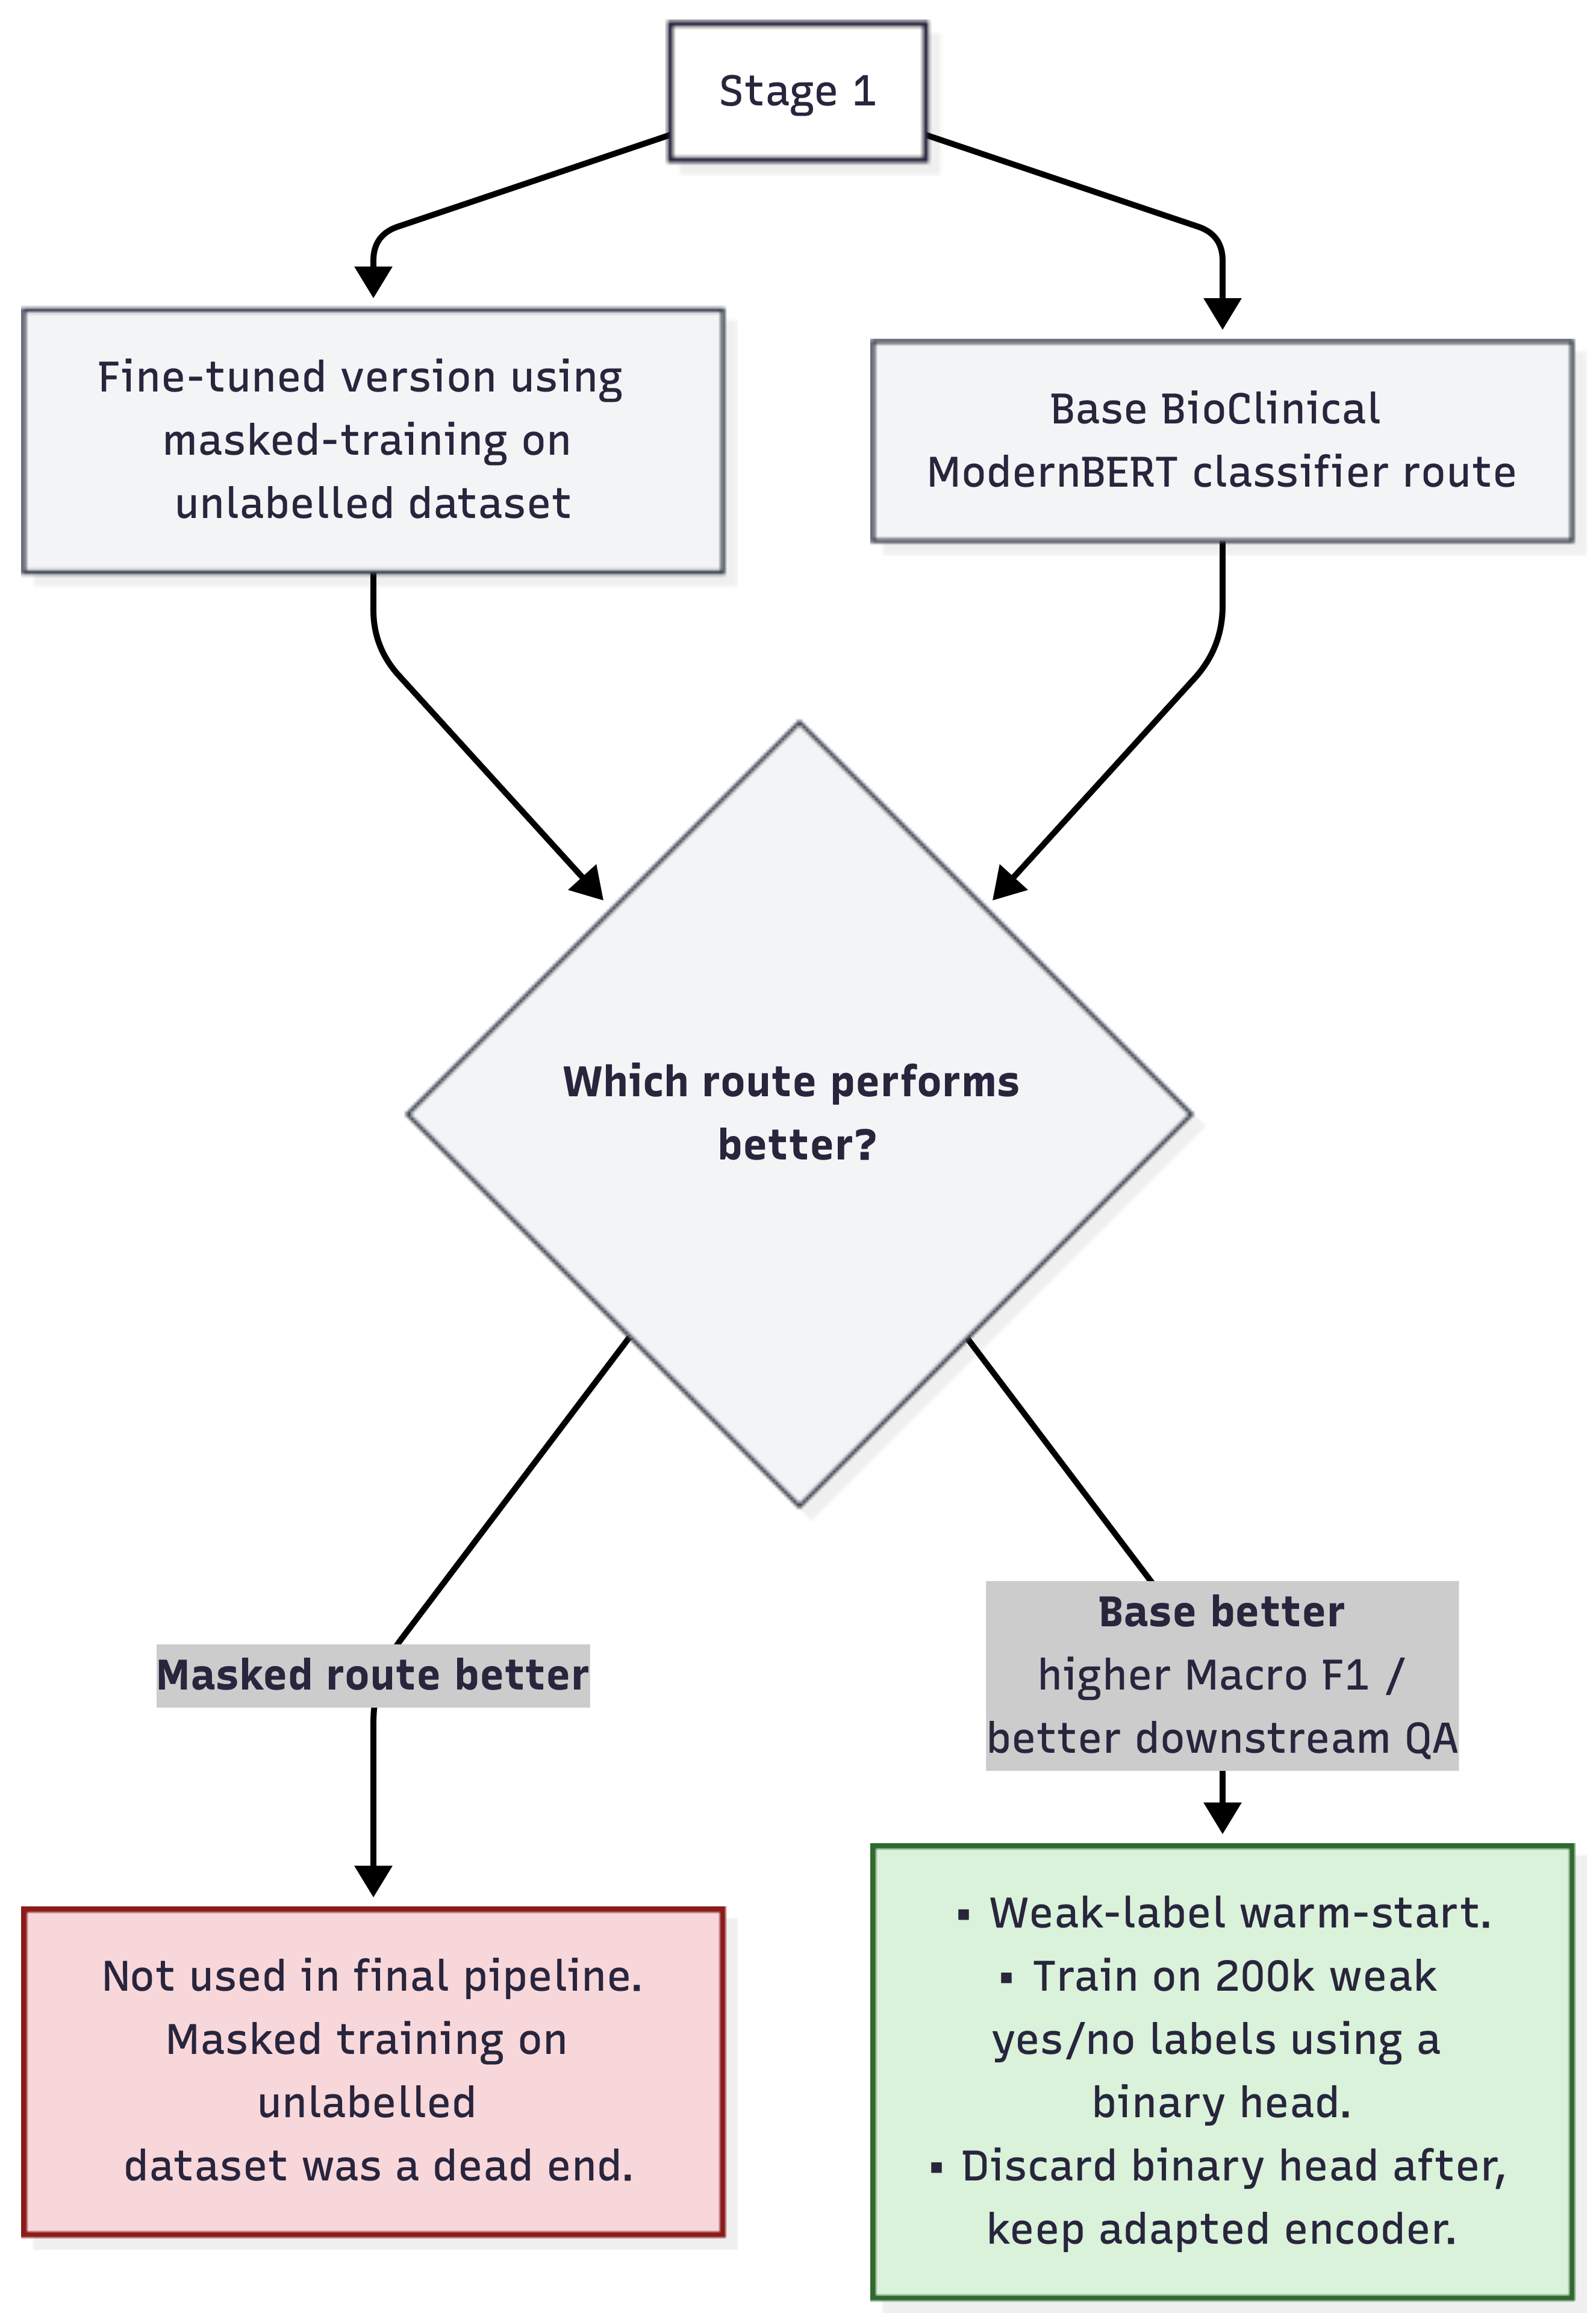
\includegraphics[width=\linewidth,height=0.82\textheight,keepaspectratio]{images/Stage1_AI.png}
        \caption{Stage~1 route selection and weak warm-start.}
        \label{fig:app_stage1_bcb}
    \end{subfigure}
    \hfill
    \begin{subfigure}[t]{0.47\linewidth}
        \centering
        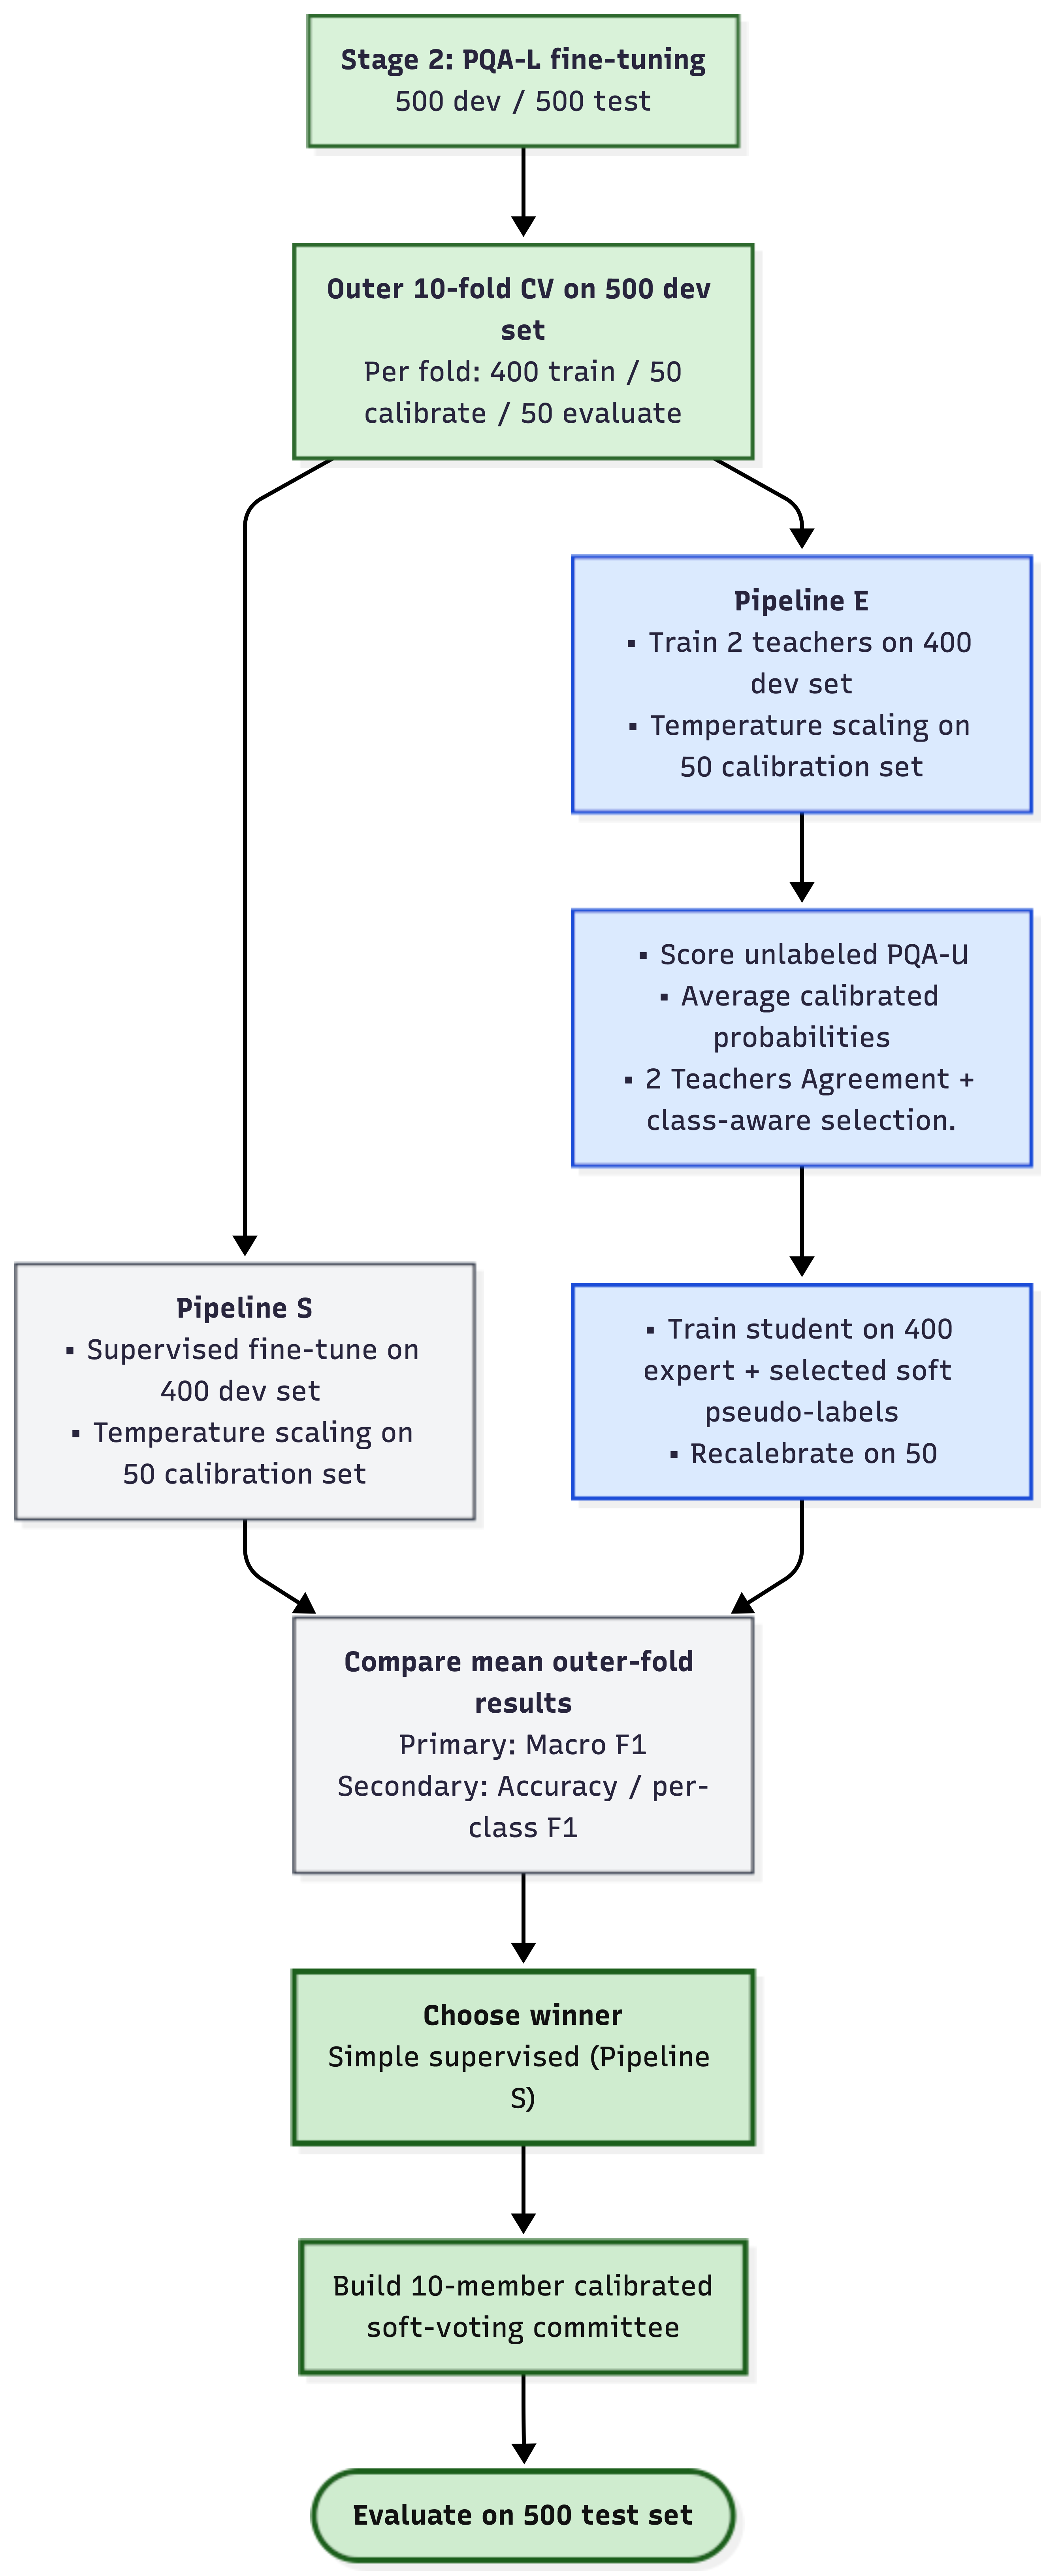
\includegraphics[width=\linewidth,height=0.82\textheight,keepaspectratio]{images/Stage2_AI.png}
        \caption{Stage~2 standardised 500/500 evaluation protocol.}
        \label{fig:app_stage2_bcb}
    \end{subfigure}
    \caption{BioClinical ModernBERT training schematics.}
    \label{fig:app_bcb_schematics}
\end{figure}